\chapter{基于智能手机的行为识别研究概述}
\par 人体行为识别就是通过感知设备获取关于人体行为的数据,然后通过信号处理和模式识别等技术手段对用户当前行为作出识别判断,其整体流程如图\ref{basic_framework}所示。行为识别的概念在上世纪八十年代就已经被提出,而在研究初期它仅仅局限在计算机视觉领域。研究者通过使用摄像头等作为感知设备获取关于人体的图像序列或视频片段,通过图像处理等技术手段提取特征并识别用户行为。随着微电子和集成电路等技术的发展,开始出现一些小型化,功能强大的传感器,一些研究者开始关注基于可穿戴传感器的行为识别技术。基于可穿戴传感器的行为识别主要使用加速度传感器采集人体的行为数据,然后提取时域和频域等特征进而识别用户行为。

\begin{figure}[htb]
\centering
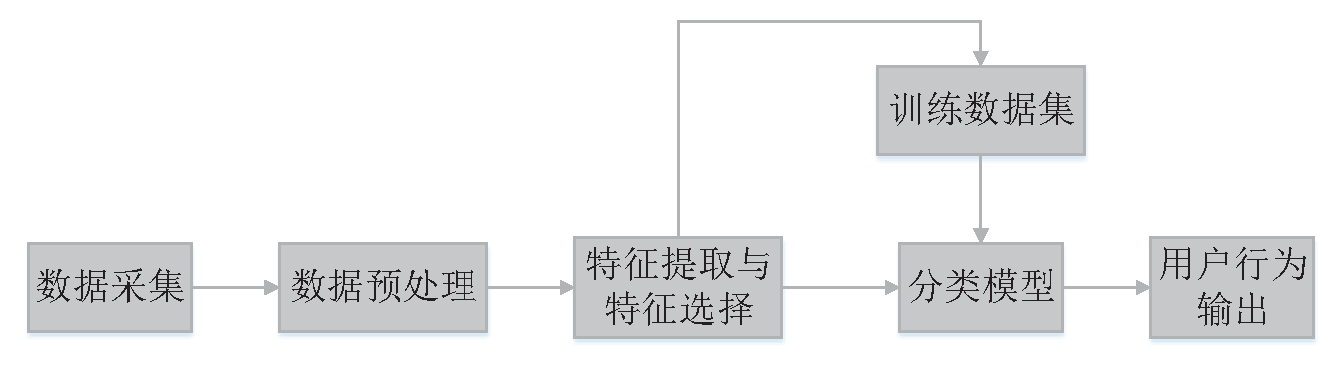
\includegraphics[width=0.8\textwidth]{basic_framework.eps}
\caption{行为识别基本框架流程图} \label{basic_framework}
\end{figure}

\par 近些年,随着智能手机的不断发展,其内部集成了越来越多的传感器,不仅包括在基于可穿戴传感器的行为识别中使用最多的加速度传感器,还包含有磁场传感器,陀螺仪等运动类型传感器,此外还有光照传感器,压力传感器,GPS等环境信息感知设备,可以获取充足的关于用户行为和环境信息。另一方面,智能手机的存储和计算能力也在不断提高与发展,其功能不断拓展与增强,这些就为基于智能手机进行行为识别提供了良好的硬件基础。伴随着智能手机的普及与应用,研究者也开始将重点关注到基于智能手机的行为识别技术。
\par 本章首先介绍智能手机内置的主要传感器以及其他感知设备,然后介绍在行为识别过程中必要的数据预处理步骤以及常用的特征提取和特征选择方法,最后详细介绍部分可以用于智能手机行为识别的分类模型和算法。

\section{数据采集}
\par 通过智能手机获取关于人体行为相关的数据一般都是通过智能手机内置传感器获取人体的加速度等信息,进而识别人体行为。本部分将首先介绍智能手机中常见的内置传感器,然后介绍智能手机中的数据采集模块。
\subsection{智能手机内置传感器}
\par 对于智能手机的内置传感器的介绍,本文以Android操作系统为例。Android操作系统是一种基于Linux的自由及开放源码的操作系统,主要用于移动设备,有Google公司和开放手机联盟领导开发。之所以选择Android系统为例介绍,一方面是因为Android是一款开源且成熟的移动端操作系统,另一方面它也也是目前市场占有量最大的手机操作系统,因此更具有代表性。对于传感器的集成以及为应用提供的传感器数据服务,其他操作系统也都十分类似,本节只是不是一般性地以Android系统为例介绍智能手机中的内置传感器。
\par Android系统平台支持的传感器类型很广泛,可以从功能和实现方式两个维度对其分类。一方面按照功能的不同,传感器可以分为运动类型传感器,环境传感器和方位传感器三类。运动类型传感器主要用于测量三轴向的加速度和角速度等,通常用于监测设备的移动,比如倾斜、震动、旋转或者摇摆等,主要包括加速度传感器、重力传感器、陀螺仪和旋转矢量传感器等。这一类型传感器在大部分智能手机内部都有集成,而且运动类型的数据也可以较好地用于人体行为识别。环境传感器则适用于测量各类环境信息参数,例如外界环境的温度、大气压强、光照强度和空气湿度等,主要包括温度传感器,气压传感器,温度传感器等。这一类型传感器在部分智能手机内有集成,可以检测人体周围环境信息,辅助人体行为识别,但是没有普适性。方位传感器主要用于测量设备的方向,主要包括磁场传感器和方向传感器,此外一般智能手机都集成了近距离创拿起,可以用于检测设备表面与物体的距离。
\par 另一方面按照实现方式的不同,传感器可以分为基于硬件和基于软件两类。基于硬件的传感器是集成在移动终端设备的物理实体。它们获得数据是通过直接测量特定的环境信息,比如加速度传感器,陀螺仪等。软件传感器是通过模拟硬件传感器,而并非真实的物理设备,它们是通过整合一个或多个硬件传感器信息相应数据,并通过一些融合方法计算获得相应模拟传感器的数据,因此也被称为虚拟传感器或者人工传感器,例如重力传感器,方向传感器等。Android平台所支持的传感器总结如表\ref{sensors}所示。

%传感器分类表
\begin{table}[htbp]
\centering
\caption{Android系统平台下内置传感器分类表} \label{sensors}
\begin{tabular}{|c|c|c|}
    \hline
    分类 & 基于硬件的传感器 & 基于软件的传感器 \\
    \hline
    运动传感器 & 加速度传感器,陀螺仪 & 线性加速度,旋转矢量传感器\\
    \hline
    环境传感器 & 光照传感器,气压传感器等 &  \\
    \hline
    方位传感器 & 磁场传感器,近距离传感器 & 方向传感器,重力传感器 \\
    \hline
\end{tabular}
%\note{这里是表的注释}
\end{table}

\par 下面本文详细介绍智能手机中常用于行为识别的传感器,包括加速度传感器,陀螺仪和磁场传感器。
\begin{itemize}
	\item 加速度传感器
\end{itemize}
\par 在Android系统平台下,存在加速度和线性加速度两类测量设备加速度,前者是基于硬件的传感器,又开发商生产直接集成在智能手机内部,产生原始的加速度数据,该数据包含重力加速度的影响。而后者则是基于软件的传感器,它是有加速度数据和其他类型传感器的数据融合后计算而得到的加速度信息,排除了重力加速度的影响。二者都会提供$x,  y,  z$三轴方向的加速度数据,其中加速度数据不仅提供加速度的大小(以$m/s^2$为单位),还提供了加速度的方向。对于每个轴向,加速度存在正值和负值分别表示两个相反方向的加速度。三个轴向的定义如图\ref{phone_orientation}所示。

\begin{figure}[ht]
\centering
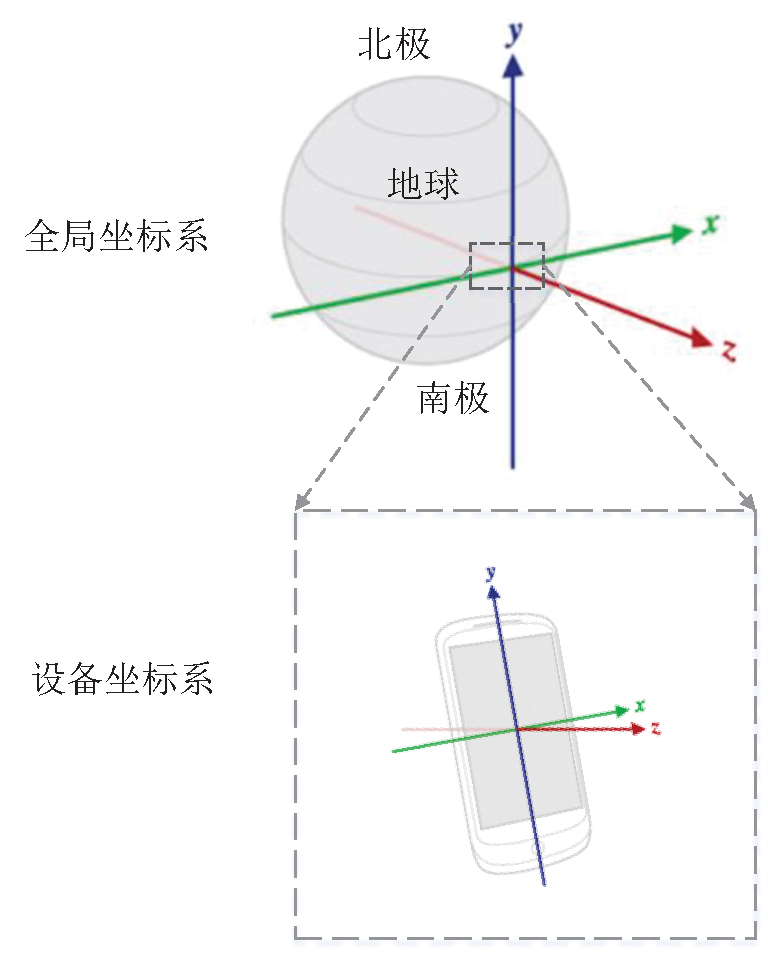
\includegraphics[width=8cm]{phone_orientation.eps}
\caption{Android全局和设备坐标系} \label{phone_orientation}
\end{figure}

\par 运动和方向传感器都是采集的矢量数据,数据的方向通常可以定义在直角坐标系中。Android系统平台定义了两个直角坐标系用以表征设备方向的相对变化。两个坐标系包括全局坐标系$x_E,  y_E,  z_E$ 以及设备坐标系$x,  y,  z$,其相对关系如图。图中表示了智能手机略微倾斜地放置在地球赤道上方时方向相对关系。在全局坐标系中$y_E$指向磁场北极,即接近正北方,$x_E$平行于地球表面,与$y_E$垂直,$z_E$指向正上方,即远离地心的方向。在设备坐标系中,$x$轴为水平方向,向右为正,$y$轴为垂直方向,向上为正,$z$轴为垂直于屏幕方向,屏幕正前方为正。几乎所有的三轴向的传感器都符合该坐标系包括下面会介绍的陀螺仪和磁场传感器,其所采集的数据均为全局坐标系中相应物理量在设备坐标系中三轴向的分解。
\par 加速度数据可以很好地表征不同行为的特点,加速度传感器在行为识别中也是应用最为广泛。基于可穿戴传感器的行为识别研究中,基于所有文献都是基于的加速度数据,而在智能手机中,加速度传感器集成也十分广泛,因此本文中它被选择为用于研究行为识别的传感器之一。

\begin{itemize}
	\item 陀螺仪
\end{itemize}
\par 陀螺仪是在设备发生旋转时,通过测量科氏(Coriolis)力测量设备在三个轴向上的角速度或旋转速度。所谓科氏力是指使得自由旋转物体从旋转参考系中看起来发生偏移的力。陀螺仪只能测量角速度,而不能直接测量旋转角度。但是可以通过陀螺仪的测量值在时间上的积分计算设备的旋转角度。陀螺仪的输出时绕设备坐标系的$x,  y,  z$三个轴向的旋转角速度值,单位为$rad/s$。如果坐标轴指向你自己,逆时针旋转则为正值,反之为负值。陀螺仪的示意图如图\ref{gyroscope}所示。

\begin{figure}[htb]
\centering
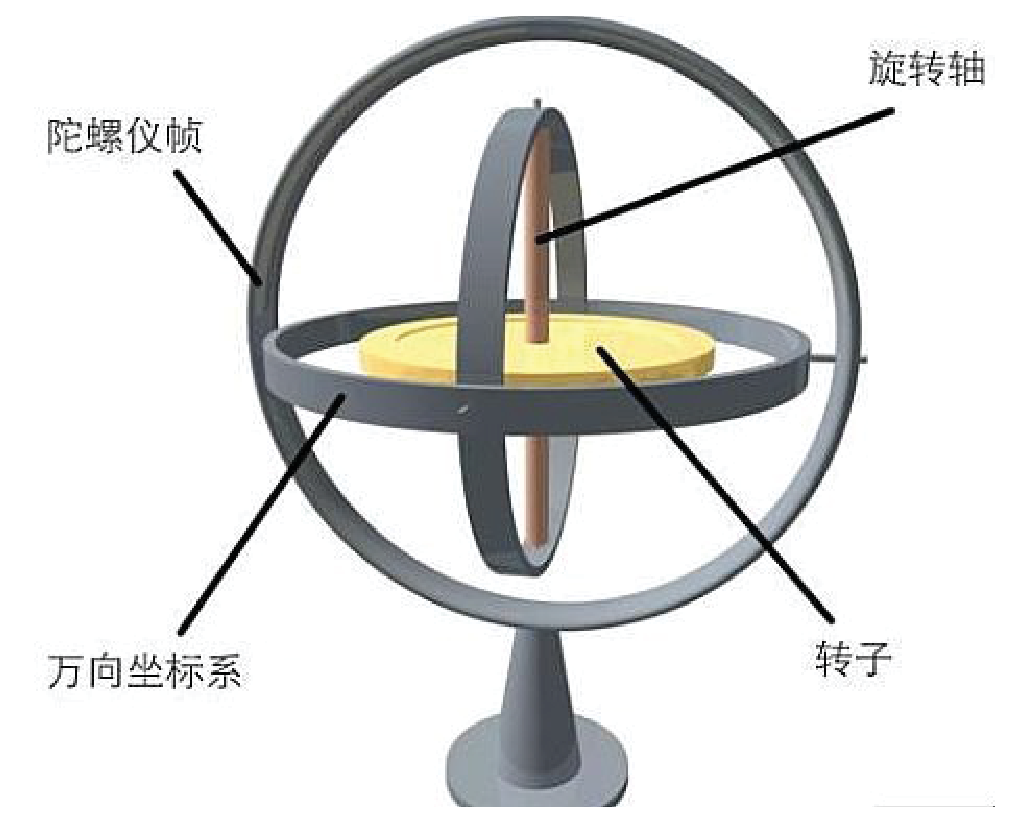
\includegraphics[width=8cm]{gyroscope.eps}
\caption{陀螺仪结构图} \label{gyroscope}
\end{figure}

\par 陀螺仪可以检测设备的旋转角速度,而在行为识别中,大部分的动态行为都是周期性行为,设备也会发生周期性旋转,所以通过处理陀螺仪数据可以很好地提取表征动态行为的特征,很好地辅助与行为识别。

\begin{itemize}
	\item 磁场传感器
\end{itemize}
\par 不同生产厂商的磁场传感器实现方式会有所不同。它们的实现方式主要可以分为基于霍尔效应、磁阻材料和洛伦兹力三种。其中霍尔效应传感器占据了最大的市场份额,在电流通过导线时,存在的磁场会使得导线两端的电子密度不同,从而形成正比于磁感应强度的电势差,通过电势差即可以计算出磁感应强度。磁场传感器也会以$x,  y,  z$三个轴向输出磁感应强度,因为集成的传感器是在每个方向上都有一个传感器。输出数据以微特斯拉$(\mu T)$为单位。
\par 磁场传感器的输出可以很好地判断设备方向的变化。在行为识别中,当行为发生转变时,磁场传感器的输出也会起到很好的辅助作用。

\subsection{智能手机数据采集模块}
\par 基于可穿戴传感器的行为识别中数据采集都是传感器将采集数据通过近距离通信的方式传送至中心节点,而基于智能手机的行为识别,其传感器和数据处理中心都是集成在手机内部,因此我们需要智能手机操作系统提供的编程接口,提取手机内置传感器的采集数据。Android系统提供了一系列的应用编程接口(Application Program Interface, API),方便获取传感器的数据。有关传感器的操作都有SensorManager负责统一管理。

\begin{enumerate}[(1)]
	\item 基本API
\end{enumerate}
\par SensorManager时Android为便于应用访问传感器数据提供的系统服务。通过SensorManager一方面可以获取手机内置的传感器对象,用Sensor类表示设备种的传感器。另一方面通过SensorManager可以允许应用注册或注销传感器相关事件,并在注册成功后可以接受传感器数据。传感器事件可以通过注册的监听器SensorEventLitener监听。注册传感器事件以获取传感器数据,需要提供对于的Sensor对象,SensorEventListener对象和数据采集的采样时间间隔等。注册成功以后即可以通过定义的SensorEventListener中的回调方法获取传感器数据。

\begin{enumerate}[(2)]
	\item 传感器采样率
\end{enumerate}
\par 在注册监听器时,通过指定监听器的采样间隔决定数据的采样率。在Android系统中,提供有四个常量表示采样间隔:SENSOR\_DELAY\_FASTEST ($0ms$,硬件传感器决定采样率),SENSOR\_DELAY\_GAME ($20ms, 50Hz$),SENSOR\_DELAY\_UI ($67ms, 15Hz$), SENSOR\_DELAY\_NORMAL ($200ms, 5Hz$)。同样也可以通过指定其他的事件间隔,即指定采样率注册事件监听器以获取相应传感器数据。

\begin{enumerate}[(3)]
	\item 传感器数据
\end{enumerate}
\par Android系统中传感器的数据是以一个SensorEvent数据结构表示,并由传感器传递至应用定义在监听器SensorEventListener中的回调方法中,从而将传感器数据传回到应用中。SensorEvent包含以下属性用以保存数据:
\begin{itemize}
	\item SensorEvent.accuracy:表示传感器当前采集数据的精度
	\item SensorEvent.senor:表示采集该数据的传感器
	\item SensorEvent.timestamp:表示采集到该数据的时间
	\item SensorEvent.values:表示传感器的数据,以数组的形式保存三轴向的数据
\end{itemize}

\section{数据预处理}
\par 首先,虽然智能手机不断发展,其内置传感器也在一直改进,但是传感器采集数据依然存在着许多噪声干扰,需要对数据做平滑和均衡处理。其次,传感器采集的关于人体行为的数据是一个连续数据流,想要通过数据流识别人体当前的行为,必然需要将其分割成一个个的数据实例,才可以对其提取特征并进一步做分类处理。因此本小节将从低通滤波和数据分段两部分介绍数据预处理的基本内容

\subsection{低通滤波}
\par 对数据的平滑和均衡处理,主要是通过低通滤波的处理,有效减少数据中的高频噪声干扰。在移动终端这个条件下,通常会采用较为滤波方法,常见的简单滤波方法有加权平滑滤波和滑动平均滤波等。

\begin{enumerate}[(1)]
	\item 加权平滑滤波
\end{enumerate}
\par 加权平滑滤波又称为一阶低通滤波,即每一个采样点的值通过上一个采样点的值与当前采样点的值取加权平均计算得到。加权平均可以实现有效阻断高频成分,保留低频信号,抑制周期性干扰,而且计算简便,易于实现。加权平均的计算公式为:
\begin{equation}
	Value[i] = Value[i-1]*(1-\alpha) + Data[i]*\alpha.
\end{equation}
其中Value表示我们计算得到的输出数值,Data表示采集的传感器数值,$\alpha$表示加权系数,决定了过去数值与当前采样数值的重要程度,位于0到1之间,起到平滑的作用。如图\ref{low_filter1}所示表示加权平滑滤波的效果。
\begin{figure}[htb]
\centering
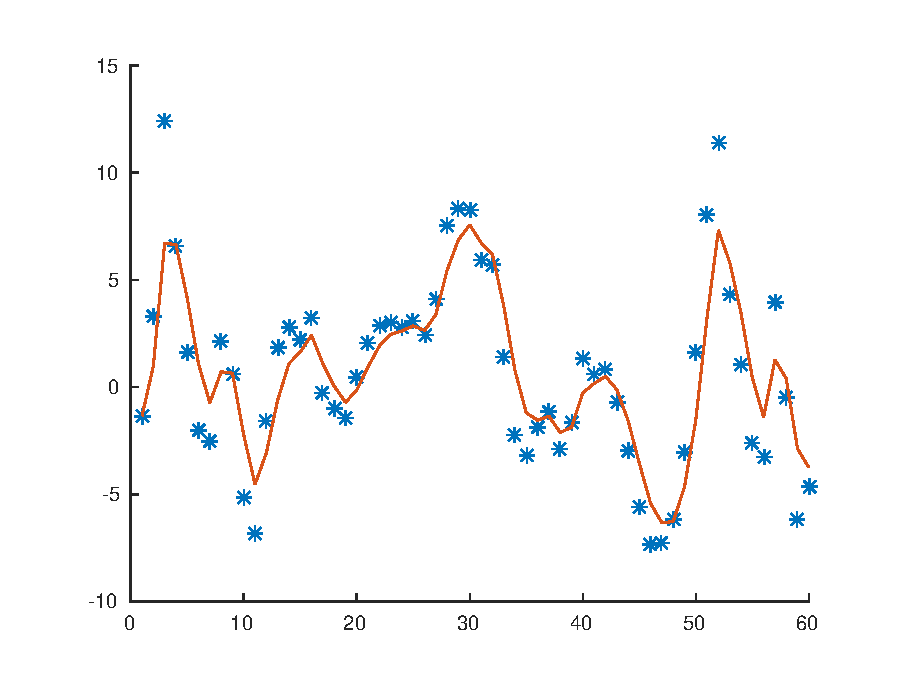
\includegraphics[width=0.6\textwidth]{low_filter1.eps}
\caption{加权平滑滤波} \label{low_filter1}
\end{figure}


\begin{enumerate}[(2)]
	\item 滑动平均滤波
\end{enumerate}

\par 滑动平均滤波就是使用过去一段时间连续采集的传感器数据,通过平均处理以后作为每个点的输出数值。这是一种常见的数字滤波方法,可以有效消除波动,降低随机噪声的干扰。同样它的计算复杂度较低,容易理解和实现,其计算公式为:
\begin{equation}
	Value[i] = \frac{1}{W}\sum_{j=0}^{W-1}Data[i-j]
\end{equation}
其中,Value为输出数值,Data为传感器原始采样数据,W为选择的用于平均处理的窗口大小。在窗口移动过程中上述公式存在着重复计算问题,为了提高计算效率,充分利用之前的计算结果,可以通过推导递推公式改进计算方式,递推公式为:
\begin{equation}
	Value[i] = Value[i-1] + \frac{1}{W}(Data[i] - Data[i-W])
\end{equation}
如图\ref{low_filter2}所示表示滑动平均滤波效果图。
\begin{figure}[htb]
\centering
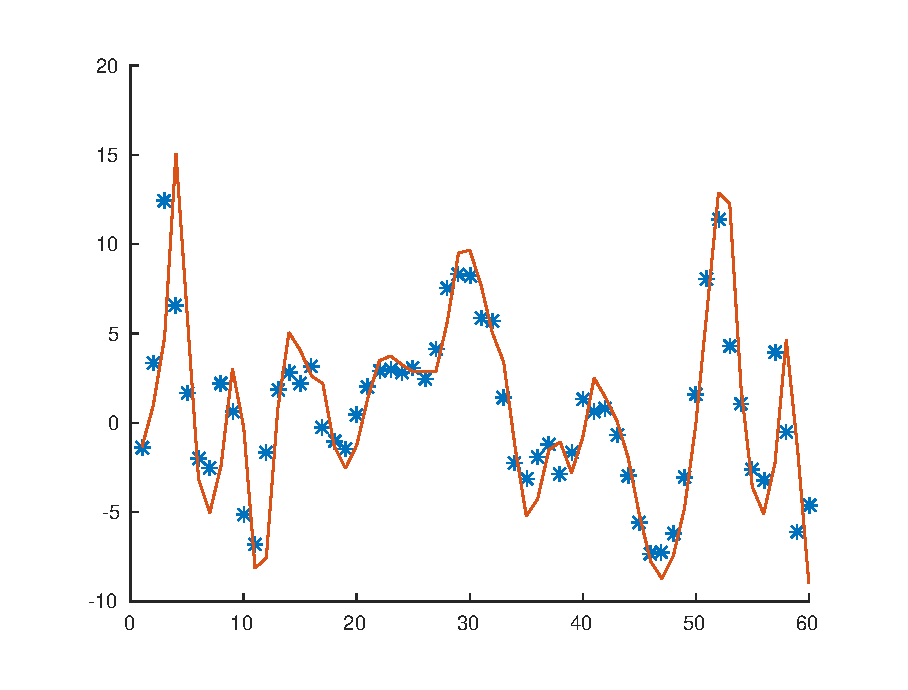
\includegraphics[width=0.6\textwidth]{low_filter2.eps}
\caption{滑动平均滤波效果图}\label{low_filter2}
\end{figure}

\subsection{数据分段}
\par 为从传感器数据流中识别人体当前的行为,有必要对连续的数据做分段处理获得行为数据实例。然后针对数据实例提取其中的部分特征进而才能通过分类算法识别出人体行为。所以分段的结果对识别结果会产生重要的影响,影响主要表现在识别准确率和识别实时性两方面。较长的数据段可以保证数据充分性提高识别准确率,而只有较短的数据段才可以保证一定的识别实时性,所以二者是一对矛盾体。为权衡二者的矛盾,重叠滑动窗口机制是在对连续数据流进行分段的常用方法。
\par 使用滑动窗口机制对数据做分段处理需要确定两个重要的参数,首先是窗口大小,其次是重叠比例。研究者通过对比实验研究了窗口大小对识别结果的影响程度。当窗口长度低于一定程度,识别准确率会随着窗口长度减小有明显下降趋势。另外一方面,重叠的比例也会影响识别实时性。较高的重叠比例可以在满足数据充分性的同时提高实时性,但是在行为转变过程中,识别反应过程就会变长,因此重叠比例也是一个需要重点考虑的参数。目前基于可穿戴传感器和基于智能手机的行为识别研究中,大部分的窗口长度都选择在3到10s之间,而重叠比例多数会选择50\%这样一个中间值。

\section{特征提取与特征选择}
\par 特征提取与特征选择对于行为识别是极其重要的一环,特征集的好坏直接决定了分类结果中识别准确率的高低。好的特征应当比较准确地表征某一类行为的一方面特点,同时该特征在不同行为之间应当表现出一定的区分度。因此,在分类之前,需要从连续的传感器数据流中提取出一系列的特征,同时还需要从这一系列特征中选择一个最佳的特征集,用于分类算法对该行为实例进行分类。本小节将从特征提取和特征选择两个步骤介绍它们通常用到的技术方法。

\subsection{特征提取}
\par 运动类型传感器所采集的关于人体行为的数据,通常都具有一定的波动性和周期性。因此基于传感器的行为识别,针对加速度等数据一般都会提取时域和频域特征,以及不同轴向数据的相关性,进而研究不同的行为特点。下面从时域和频域两个方面介绍常用特征。

\begin{enumerate}[(1)]
	\item 时域特征
\end{enumerate}
\par 时域特征通过时域信号直接计算得到,计算简单,复杂度低。时域特征通常包括均值、均方根、方差、标准差、最值、相关系数等。

\par 均值($\overline{X}$)和均方根(Root Mean Square, RMS)描述了传感器数据在一个窗口时间内的平均大小,代表传感器数据的直流分量,体现了时域信号的低频特性。它们的计算公式如下:

\begin{equation}
	\overline{X} = \frac{1}{N}\sum_{i=1}^{N}x[i]
\end{equation}
\begin{equation}
	RMS(X) = \sqrt{\frac{1}{N}\sum_{i=1}^{N}x[i]^2}
\end{equation}
\par 方差($\sigma_X^2$)和标准差($\sigma_X$)描述了传感器数值分布的离散程度,体现了运动传感器信号的稳定性,方差计算公式如下,标准差为方差的算术平方根。

\begin{equation}
	\sigma_X^2 = \frac{1}{N-1}\sum_{i=1}^{N}(x[i]-\overline{X})^2
\end{equation}
其中,$\overline{X}$表示$X$轴向上窗口时间内传感器数据的均值,$N$为窗口时间内数据采样点数。
\par 相关系数($r_{XY}$)是一个常用统计量,常用于衡量变量之间的线性相关程度。传感器的不同轴向的数据之间的相关系数可以很好地表征行为的运动模式,可以用于区分不同的运动行为。$X$与$Y$轴的相关系数的计算公式如下:

\begin{equation}
	r_{XY} = \frac{\sum_{i=1}{N}(x[i] - \overline{X})(y[i] - \overline{Y})}{\sqrt{(x[i] - \overline{X})^2}\sqrt{(y[i] - \overline{Y})^2}}
\end{equation}
其中,$\overline{X}$和$\overline{Y}$分别表示$X$,$Y$轴向上窗口时间内传感器数据的均值,$N$为窗口时间内数据采样点数。
\par 此外时域特征还包括最大值、最小值、四分位距、分布直方图等,这里不再一一介绍。

\begin{enumerate}[(2)]
	\item 频域特征
\end{enumerate}
\par 频域特征可以表现运动行为的周期性特点,通常需要先对时域信号做快速傅里叶变换(Fast Fourier Transform, FFT),然后再对频域信号计算频域特征值。频域的特征通常包括频域的最值、频谱能量、频域熵、功率谱密度等。
\par 频谱能量($Energy$)描述运动状态下,传感器信号的周期特性,其计算方式为对快速傅里叶变换后的频谱序列各个分量的幅度计算平方和,其计算公式如下:
\begin{equation}
	Energy(X) = \frac{\sum_{i=1}^{N}|F_i|^2}{N}
\end{equation}
其中,$|F_i|$是信号频谱中的第$i$个分量的幅度。
\par 信息熵($Entropy$)描述信号频谱特征,其计算方式同样是对快速傅里叶变换后的频谱序列,对其求取信息熵,反应频谱的分布特征,其计算公式如下:
\begin{equation}
	Entropy(X) = \sum_{i=1}^{N}(-p_ilogp_i)
\end{equation}
其中,$p_i$表示信号频谱中第$i$个分量在频谱中所占的比例。
\subsection{特征选择}
\par 通过一系列的特征计算,可以组成关于一段窗口时间内数据的特征向量。如果特征向量中特征数量太多,一方面需要消耗大量的计算资源,另一方面还会在训练分类模型中造成过拟合导致人体行为识别准确率下降。因此我们需要从可选特征向量中选择最佳特征集用于训练分类模型以及行为实例的分类。特征选择方法很多,使用较为广泛的主要包括主成分分析法,线性判别分析法以及根据信息增益特征排序选择方法等。
\par 主成分分析(PCA),就是通过正交变换,将原来存在一定相关性的特征向量变换为在分量上不相关的随机向量。具体地,首先计算特征向量的协方差矩阵而转换为一个对角矩阵,然后对其做正交变换,将其变换到$p$个正交方向,从而将多维的特征向量降为低维向量,而且尽可能多地保留信息,从而达到降维的效果。
\par 线性判别分析法(LDA),其基本思想是将高维的特征向量映射到最优的矢量空间,然后抽取分类信息以及降低特征空间的维数。通过映射以后的特征空间具有最优的可分离性,在新的子空间中具有最小的类内距离和最大的类间距离。最终在降低特征维度以后获得最佳的分类效果。
\par 另外一种常用的方法就是使用有监督的方法计算每一维特征的信息增益或信息增益比,进而对所有特征排序,然后选择信息增益或信息增益比最大的若干特征组成特征集。信息增益(information gain, IG),其计算公式如下:

\begin{equation}
	Entropy(t) = -\sum_{i=1}^{c}p(i|t)log_2p(i|t)
\end{equation}
\begin{equation}
	IG = Entropy(parent) - \sum_{j=1}^{k}\frac{N(v_j)}{N}Entropy(v_j)
\end{equation}
其中,$Entropy(.)$表示信息熵,$t$表示记录总数,$c$表示类别总数,$p(i|t)$表示类型$i$记录数所占的比例;在公式2.10中,$k$表示属性值的个数,$N$表示记录总数,$N(v_j)$表示按照某特征分类,实例被分为$j$类的实例数量。因此信息增益其实就是按照某一个特征对所有实例分为$k$类,分类前后信息熵的差值。
这种方法计算简单且易于理解,尽可能地保留了特征空间中不同类别行为之间的区分度,选择的特征集可以较好地用于分类模型。

\section{分类算法}
\par 所谓人体行为识别就是根据一定时间的行为特征判断这段时间最有可能的行为,可以将其归结为分类问题。从数据挖掘和模式识别的角度看,行为识别就是一个多分类的问题。在模式识别领域存在着诸多的成熟分类算法,本小节将从基础分类算法和提升分类算法两部分介绍常用于人体行为识别的分类算法。

\subsection{基础分类算法}
\par 基础分类算法由于其算法简单易于实现,而且算法复杂度较低,因此需要在智能手机终端对行为作出识别判断的研究中,这类算法应用特别广泛。常用于基于智能手机的行为识别研究中的基础分类算法主要包括K-近邻分类算法,朴素贝叶斯算法,决策树和支持向量机等。

\begin{itemize}
	\item K-近邻分类算法(K-Nearest Neighbor, KNN)
\end{itemize}
\par K-近邻分类算法是一种有监督的惰性机器学习算法。该算法简洁且易于理解,其基本思想就是在特征空间中定义一种实例之间的距离,使用最多的时欧氏距离,当有实例需要判定类别时,在所有实例中按照定义好的特征空间距离寻找K个与之距离最短的实例,根据这K个实例的标签决定该实例的类别。KNN的算法的优点是简单易于实现,且不需要训练分类模型,但也有一定的缺点。使用KNN必须保存一定数量的实例,占用一定的存储空间,而且它是一种惰性分类算法,需要在识别时计算实例之间的距离,可能会对识别实时性造成一定影响。
\begin{itemize}
	\item 朴素贝叶斯分类算法(Naive Bayesian)
\end{itemize}
\par 朴素贝叶斯分类算法是基于贝叶斯定理之上实现的有监督的学习算法,贝叶斯定理如下:
\begin{equation}
	P(H|X) = \frac{P(X|H)P(H)}{P(X)}
\end{equation}
其中,$H$表示一种假设,在分类模型中表示分为某一类的假设,$X$表示支持该假设的证据,在分类模型中表示特征向量的某一个特定取值组合, $P(X)$和$P(H)$时$X$和$H$的先验概率,$P(X|H)$是在$H$条件下$X$的条件概率。
\par 朴素贝叶斯分类算法的基本假设是所有特征彼此独立。因此条件概率可以同以下方法计算:
\begin{equation}
	P(X|H) = \prod_{k=1}^{n}P(x_k|H)
\end{equation}
其中,$x_k$表示第$k$个属性的值。
由于先验概率容易获得,而条件概率计算以后就可以计算获得一个特征组合下,每一个假设分类的后验概率,通过比较选择最大后验概率即可获得分类结果。朴素贝叶斯分类算法同样简单易于实现,但是最大的限制就在于对特征彼此独立的假设条件。

\begin{itemize}
	\item 决策树(Decision Tree)
\end{itemize}
\par 决策树是一种有监督的学习分类算法,其分类的流程实例如图\ref{decision_tree}所示。决策树的每个叶节点代表一个类别,每个分支代表一个组属性值组合。决策树的建立时基于实例数据的信息熵。每一步的数据实例分裂都选择使得信息增益或信息增益比最大的特征将数据实例分裂为若干类,直到将所有实例都分类。为了避免出现过拟合,决策树中还可以通过剪枝的方法泛化模型。决策树最大的优势就是易于理解分类规则,易于实现,而且不依赖于特征的独立性,所以较为广泛地应用在行为识别当中。

\begin{figure}[!htb]
\centering
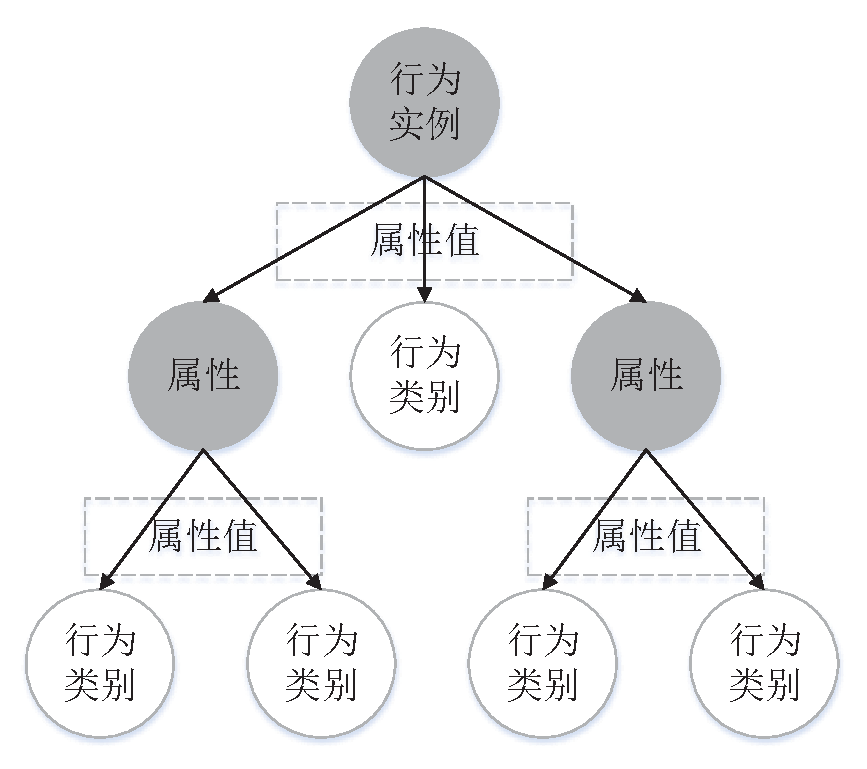
\includegraphics[width=8cm]{decision_tree.eps}
\caption{决策树分类算法流程图} \label{decision_tree}
\end{figure}
\begin{itemize}
	\item 支持向量机(Support Vector Machine, SVM)
\end{itemize}
\par 支持向量机是一种最为常用的有监督学习算法,它通过计算一个或多个高维的超平面将实例数据分割成多个类,其原则是使得超平面与支持向量的间隔最远。对于线性可分情况,可以直接计算超平面用于分类,对于线性不可分情况可以使用非线性映射算法将低维输入线性空间映射到高维的特征空间,使其线性可分,然后求解超平面对其进行分类。支持向量机同样广泛应用与行为识别,姿势识别等领域。

\subsection{提升分类算法}
\par 由于智能手机的计算能力有限以及行为识别对实时性的要求,基于智能手机的行为识别研究中,提升的分类算法应用并不太广泛,这里只介绍随机森林分类算法。随机森林计算相对简单,复杂度相对较低,而且一些研究者也通过实验表明该学习方法在行为识别中取得了很好的效果。
\begin{itemize}
	\item 随机森林分类算法(Random Forest)
\end{itemize}
\par 随机森林分类算法是决策树的一种组合形式。在随机森林的建立阶段,从$M$个特征中随机选择$m$个特征,其中$m<<M$,使用这$m$个特征建立决策树,其过程与独立决策树完全相同。多次执行相同过程,这些随机选择特征集的决策树就组建成了随机森林。在决策分类阶段,实例会通过每一棵决策树进行分类,最终的结果由所有决策树的分类结果投票决定。
\par 随机森林在建立阶段一方面由于随机选择少量特征,不容易出现过拟合,而且训练速度较快,计算复杂度相对较低,另一方面是从特征集中随机选择特征,因此也可以用于高维特征数据实例的分类,而且对特征选择的要求不高。同时,在决策分类阶段,由于综合了多个决策树的结果,在准确率上有了很大的提高,在应用到行为识别上,这一点在文献中通过实验获得了证实。

\section{本章小结}
\par 本章简要介绍了基于智能手机行为识别的相关技术。首先简要概述了智能手机中内置传感器种类和功能以及手机的数据采集模块。然后介绍了数据预处理方法,包括低通滤波和数据分段处理,同时介绍了行为识别中常用特征以及特征选择方法。最后介绍了可以用于基于传感行为识别的分类算法